\section{Systemanalyse im Frequenzbereich}
    \subsection{Laplace-Transformation}
    \begin{center}
        {\renewcommand{\arraystretch}{1.5}
        \begin{tabular}{l | l}
        \multicolumn{2}{l}{\textbf{Wichtige Eigenschaften:}}\\
            \hline
            Linearität  & $\mathcal{L}\{a x_1(t)+b x_2(T)\} = a X_1(s)+b X_2(s)$\\
            Ähnlichkeit & $\mathcal{L}\{\frac{1}{a}\cdot x(\frac{t}{a})\} =X(s\cdot a) $ \\
            Verschiebung & $\mathcal{L}\{x(t-T)\} = e^{-T\cdot s} \cdot X(S)$ \\
            Dämpfung & $\mathcal{L}\{(x(t)\cdot e^{a\cdot t}\} = X(s-a)$\\
            Ableitung t & $\mathcal{L}\{\frac{d}{dt}x(t)\} = s \cdot X(s) - x(0)$\\
            $n-$te Abl. t & $\mathcal{L}\{\frac{d^nx(t)}{dt^n}\} = s^n \cdot X(s)(\frac{d^kx(t=0)}{dt^k}= 0 \forall k)$\\
            Ableitung s & $\mathcal{L}\{t\cdot x(t)\} = -\frac{d}{ds}X(s)$\\
            Integration t & $\mathcal{L}\{\int_0^t x(\tau)d\tau\} = \frac{1}{s}\cdot X(s)$ \\
            Integration s &  $\mathcal{L}\{\frac{1}{t}\cdot x(t)\} = \int_s^\infty X(\sigma)d\sigma$ \\
            Faltung t & $\mathcal{L}\{x_1(t)*x_2(t)\} = X_1(s) \cdot X_2(s)$ \\ 
            Anfangswert & $\displaystyle\lim_{t \to 0^{+}}x(t) =\lim_{s \to \infty}s\cdot X(s)$ \\
            Endwert & $\displaystyle\lim_{t \to \infty}x(t) =\lim_{s \to 0}s\cdot X(s)$
             
        \end{tabular}}
    \end{center}
    
    \begin{center}
        {\renewcommand{\arraystretch}{1.4}
        \begin{tabular}{c|c}
        \multicolumn{2}{l}{\textbf{Wichtige Singaltransformationen:}}\\
            \hline
            $x(t)$ & $X(S)$ \\
        \hline
            $\delta(t)$ & $1$\\
            $h(t)\quad(=1)$ & $\frac{1}{s}$ \\
            $p(t)\quad(=t)$ & $\frac{1}{s^2}$ \\
            $h(t) \cdot t^n \cdot e^{\alpha\cdot t}$ & $\frac{n!}{(s-\alpha)^{n+1}}$ \\
            $h(t) \cdot sin(\omega\cdot t)$ & $\frac{\omega}{s^2 + \omega^2}$\\
            $h(t) \cdot cos(\omega\cdot t)$ & $\frac{s}{s^2+\omega^2}$\\
            $h(t)\cdot sinh(\omega\cdot t)$ & $\frac{\omega}{s^2-\omega^2}$\\
            $h(t) \cdot cosh(\omega\cdot t)$ & $\frac{s}{s^2-\omega^2}$\\
            $h(t) \cdot (e^{at}-1)$&$ \frac{a}{s(s-a)}$\\
            $h(t) \cdot \frac{e^{at} - e^{bt}}{a-b}$ & $ \frac{1}{(s-a)(s-b)}$ \\
            $h(t) \cdot \frac{ae^{at} - be^{bt}}{a-b}$ & $ \frac{s}{(s-a)(s-b)}$
        \end{tabular}} 
    \end{center}
    
        \subsubsection{Anwendungen}
            \textbf{Übertragungsfunktion:}
            
            Da Ableitungen im Zeitbereich zu algebraischen Grössen im Frequenzbereich werden. Lässt sich die Lösung einer Zustandsgleichung erster Ordnung folgendermassen finde:
             \[
             \dot{x}(t) = A \cdot x(t) + b \cdot u(t), \hspace{4mm} y(t) = c \cdot x(t), \hspace{4mm} x(0) = 0 \]
             \[
            \Downarrow{\mathcal{L\{\}}}
            \]
            \[
            s\cdot X(s) = A \cdot X(s) + b\cdot U(s), \hspace{3mm} Y(s) = c\cdot X(s)
            \]
            \[
            \Downarrow{Umformen}
            \]
            \[
            Y(s) = c\cdot (sI-A)^{-1}\cdot b \cdot U(s) = \Sigma(s) \cdot U(s)
            \]
            Wobei $\Sigma(s)$ Übertragungsfunktion heisst, $\Sigma(s)$ ist im Allgemeinen ein Bruch rationaler Funktionen, wobei der Nenner bei physikalischen Systemen mindestens die Ordnung des Zählers hat ($n \geq m$)
            \[\Sigma(s) =   \frac{Y(s)}{U(s)} =\frac{c\cdot \textrm{Adj}(s\mathbb{I}-A)\cdot b}{\textrm{det}(s\mathbb{I} -A)}+d\]
            \[
            = \frac{b_m\cdot s^m+ \hdots + b_1 \cdot s + b_0}{s^n + a_{n-1}\cdot s^{n-1}+\hdots + a_1\cdot s^{1} + a_0} +d\]
            Der Nenner $det(sI-A)$ entspricht der charakteristischen Gleichung der Matrix A. D.h. Stabilitätseigenschaften der GGWP lassen sich am Nenner ablesen.
        
            \textbf{Adjunkte berechnen}
            
            Die Adjunkte für eine $2 \times 2 $-Matrix berechnet sich folgendermassen. 
            \[
            A = \begin{bmatrix}
            a & b \\ c & d
            \end{bmatrix}
            \xRightarrow{adjungieren}
            \textrm{Adj}(A) = \begin{bmatrix}
            d & -b \\ -c & a
            \end{bmatrix}
            \]
            
            \textbf{Anfangs- und Endwerte:}
            
            lässt sich mithilfe des Anfangs-/Endwerttheorem im Frequenzbereich berechnen.
            \[Y(s)=\Sigma(s)\cdot U(s), \quad U(s) = \mathcal{L}\{h(t)\} = \frac{1}{s}\]
            \[\Rightarrow Y(s)=\Sigma(s)\cdot\frac{1}{s}\]
            \[y(0_+) = \lim_{s\to\infty}s\cdot Y(s)=\lim_{s\to\infty}\Sigma(s)\]
            \[y(\infty) = \lim_{s\to0_+}s\cdot Y(s)=\lim_{s\to0_+}\Sigma(s)\]
            
            \textbf{Übertragungsfunktionen haben die allgemeine Form:}
            \[\Sigma(s)=b_m\cdot\frac{\prod_{j=1}^{m}(s-\xi_j)}{\prod_{i=1}^{n}(s-\pi_i)}, \quad \xi_j,\pi_i \in \mathbb{C}\]
            wobei $\pi_i$ Pole und $\xi_j$ Nullstellen genannt werden. Jeder Pol $\pi_i$ entspricht einem Eigenwert $\lambda_i$ von $A$. 
            \\\textbf{Vorsicht:} Nicht alle Eigenwerte von $A$ sind Pole $\pi_i$ von $\Sigma(s)$, da sich Nullstellen und Pole kürzen können! Wenn die Übertragungsfunktion aus einer minimalen Systemrealisierug $\{A,b,c,d\}$ berechnet wird, lassen sich keine Pole und Nullstellen aufheben. \textbf{Das Kürzen von Termen ist somit ein Hinweis dafür, dass das System }$\{A,b,c,d\}$\textbf{ nicht beobachtbare oder nicht steuerbare Zustände enthält.} Diese Zustände beeinflussen das I/O-Verhalten nicht.
            
    
    \subsection{Inverse Laplace-Transformation}
        \[y(t)=\mathcal{L}^{-1}\{Y(s)\}=\frac{1}{2\pi j}\oint Y(s)\cdot e^{s\cdot t}ds \quad t>0\]
        Sehr schwer zum Ausrechnen. Da Lösungen im Frequenzbereich gebrochene rationale Funktionen sind:
        \[Y(s)=b_m\cdot\frac{\prod_{j=1}^{m}(s-\xi_j)}{\prod_{i=1}^{n}(s-\pi_i)}, \quad \xi_j,\pi_i \in \mathbb{C}\]
        Insbesondere kann man mit der Partialbruchzerlegung den Bruch in eine Linearkombination von Brüchen tieferer Ordnung zerteilen:
        \[Y(s)=\sum_{i=1}^{p}\sum_{k=1}^{\phi_i}\frac{\rho_{i,k}}{(s-\pi_i)^k} \quad \rho_{i,k}\in\mathbb{C}\]
        wobei $\rho_{i,k}$die Residuen sind und $\phi_i$ die Vielfachheit von $\pi_i$ ist. Die inverse Laplace-Transformation der einzelnen Brüche kann allgemein hergeleitet werden:
        \[\mathcal{L}^{-1}\left\{\frac{1}{(s-\pi_i)^k}\right\}=\frac{1}{(k-1)!}\cdot t^{k-1}\cdot e^{\pi_i\cdot t}\cdot h(t)\]
        
        \subsubsection{Bsp}
            \[Y(s)=\frac{s^2+s+2}{s^3+s^2+s+1}=\frac{s^2+s+2}{(s+j)(s-j)(s+1)}\]
            \[Y(s)= \frac{1}{s+1}+\frac{\frac{1}{2j}}{s-j}+\frac{-\frac{1}{2j}}{s+j}\]
            \[\mathcal{L}^{-1}=y(t)= e^{-t}+\frac{1}{2j}\left(e^{j\cdot t}-e^{-j\cdot t}\right)= e^{-t}+\sin{t}\]
    
    \subsection{Systeme 2. Ordnung}
        Die Übertragungsfunktion eines Systems zweiter Ordnung mit statischer Verstärkung von 1 hat folgende Form:
        \[\Sigma(s) = \frac{\omega_0^2}{s^2 + 2 \cdot \delta \cdot \omega_0\cdot s + \omega_0^2} \hspace{4mm} \Sigma(0) = 1
        \]
        Dieses System hat zwei Pole: 
        \[
        s_{1,2} = \pi_{1,2} = (-\delta \pm \sqrt{\delta^2-1}) \cdot \omega_0
        \]
        Anordnung der Pole auf der real-imaginären Ebene:
        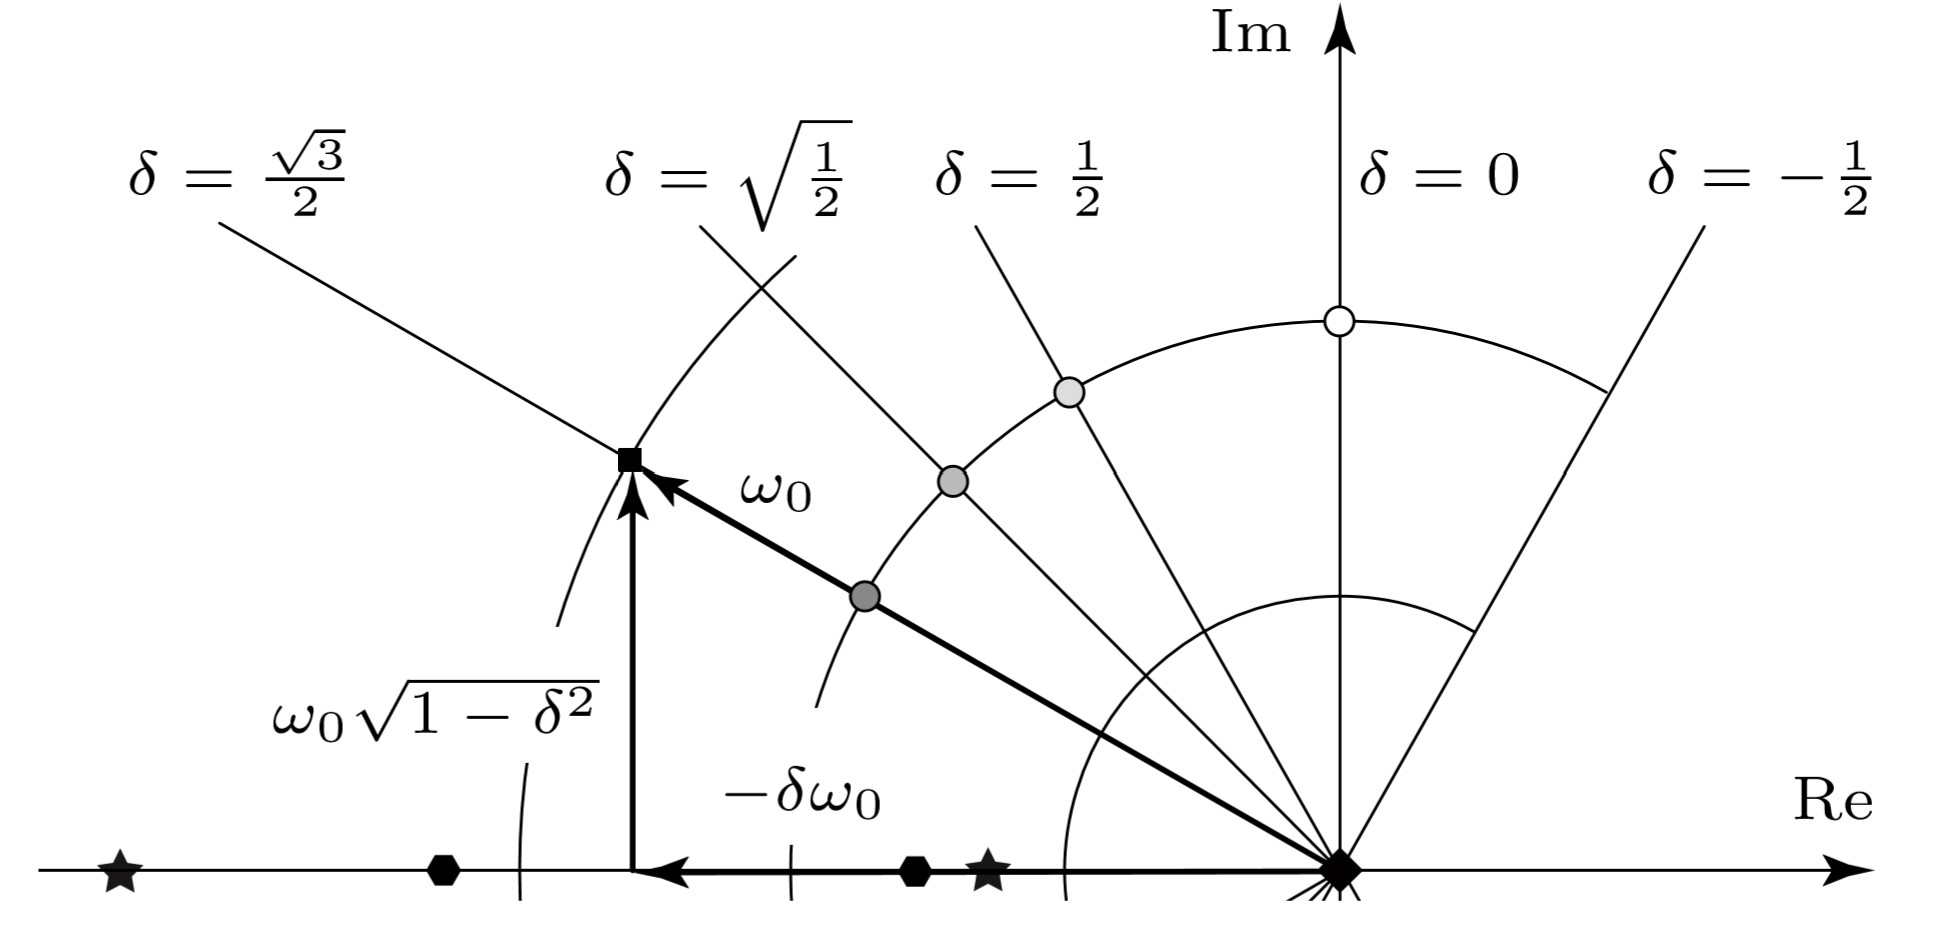
\includegraphics[width=\linewidth,height=45mm]{images/04/Anordnung_Polstellen.jpg}
        
        Dabei ist $\delta$ der \textbf{Dämpfungsparameter}. 
        Für $| \delta | < 1$ sind die Pole komplex.
        Für $| \delta | > 1$ sind die Pole rein reell.
        
        $\omega_0 = 2\pi/T_0$ ist die \textbf{natürliche Frequenz}, wobei $T_0$ die \textbf{natürliche Periode} ist.
        
        Abhängig von der Dämpfung gibt es drei grundsätzlich unterschiedliche Fälle des Systemsverhalten:
        
        $\boxed{ 0 < \delta < 1 }$  System enthält \textbf{Schwingungen}. 
        Die erste Schwingung überschiesst das Ziel $u(t) = h(t)$ um den Überschuss $\hat{\epsilon} = e^{-\delta\cdot\pi/\sqrt{1-\delta^2}},$ bei der Zeit $t^* =\frac{\pi}{\omega_0\cdot\sqrt{1-\delta^2}}$
        
        $\boxed{\delta > 1}$ Für \textbf{ungedämpfte Systeme} konvergiert das System, ähnlich wie bei einem System erster Ordnung zum Endwert. Die Systemantwort überschiesst in diesem Fall nicht. 
        
        $\boxed{ \delta = 1}$ Dieser Fall heisst \textbf{kritisch gedämpft} und entspricht der schnellst möglichen Konvergenz ohne Überschwinger.
        
        \begin{center}
            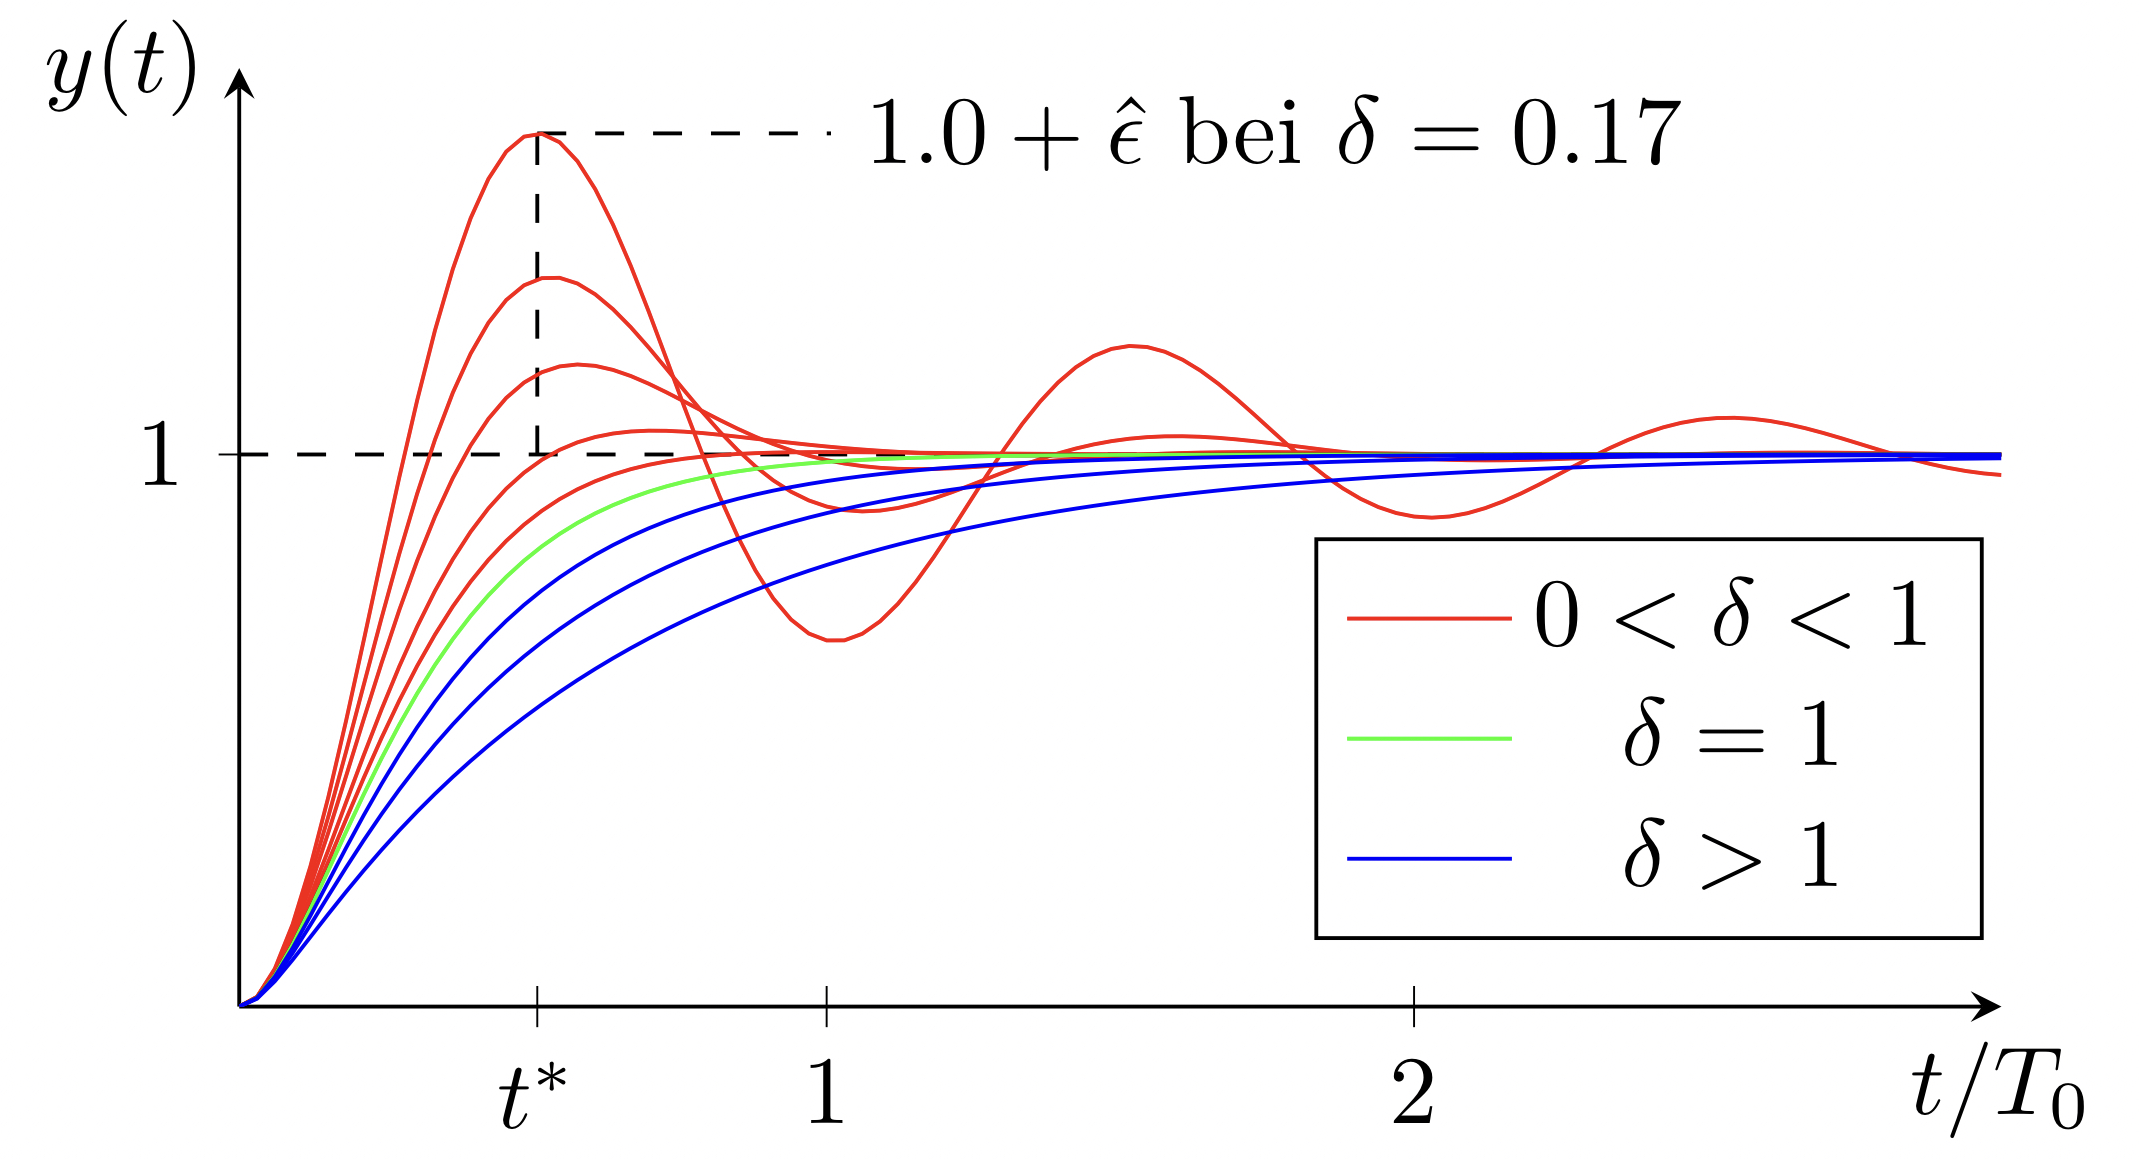
\includegraphics[width=0.55\linewidth]{04/dampening_sys_2.jpeg}
        \end{center}
        
        \subsubsection{Bsp Vereinfachung für $\delta>1$}
            \[\Sigma(s)= \frac{100}{s^2+101s+100}= \frac{100}{(s+100)(s+1)}\]
            Impulsantwort hat die Form: $\alpha\cdot e^{-100t}+\beta\cdot e^{-t}$. Da $e^{-100t}$ viel schneller abklingt als $e^{-t}$ kann man das System approximieren:
            \[\Sigma_{\textrm{approx}}(s)=\frac{1}{s+1}\]
            Man muss den Zähler anpassen, um die statische Verstärkung des approximierten Systems gleich zu halten: $\Sigma(0)= \Sigma_{\textrm{approx}}(0)$.
            \begin{center}
                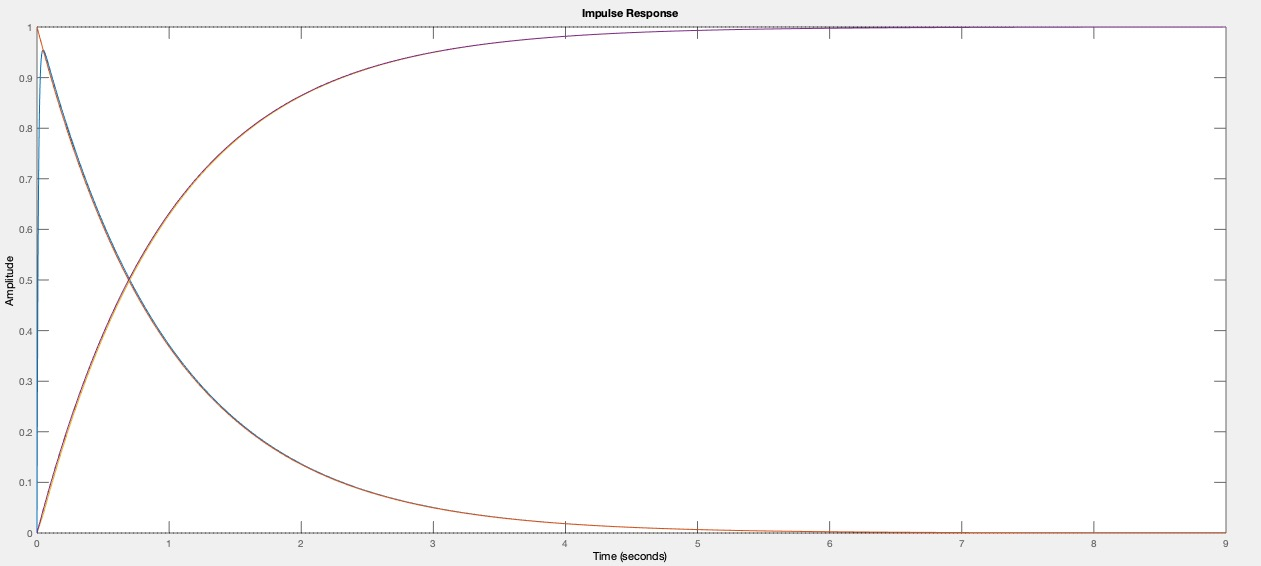
\includegraphics[width=\linewidth]{04/impulse_step_response_approx.jpg}
                \textit{Blau: Genaues System; Orange: Approximiertes System}
            \end{center}
        
        \subsection{Nullstelleneinfluss}
        \[\Sigma(s)=\frac{a\cdot s+1}{\dots}\]
        %Einfluss von Nullstellen auf das Systemverhalten.%
        Je näher die Nullstelle $\zeta = -1/a$ am Ursprung ist, desto stärker ist der Einfluss dieser Nullstelle. Dies widerspiegelt sich an einem stärkeren Überschuss in der Systemantwort. 
        Für $\zeta > 0 $ hat die Systemantwort einen \textbf{Undershoot}. Das heisst das System antwortet zuerst in die falsche Richtung. ein System mit einer Nullstelle der Form $\zeta > 0$ wird als \textbf{nicht-minimalphasig} bezeichnet.
        
        \textbf{Bemerkung:}
        Die initiale Sprungantwort in die `falsche' Richtung tritt bei einer ungeraden Anzahl positiver Nullstellen (Re($\zeta > 0))$ auf.
        \\Falls Steigung gleich 0 in $t=0$ ist, ist keine NST vorhanden
        
        \begin{center}
            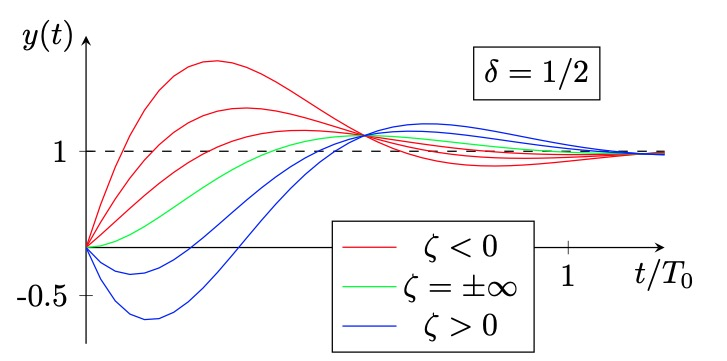
\includegraphics[width=0.8\linewidth]{04/NSTeinfluss.jpg}
        \end{center}
        
    \subsection{BIBO Stabilität}
        \textbf{BIBO} Stabilität bezieht sich auf das \textbf{I/O-Verhalten} von $\Sigma(S)$, wobei \textbf{Lyapunov Stabilität} sich auf das GGW der \textbf{Zustände} bezieht. 
        
        Ein System ist BIBO Stabil, falls für die Impulsantwort $\delta(t)$ folgendes gilt:
        \[\int_0^\infty|\delta(t)|dt < \infty\]
        \begin{itemize}
            \item Das System ist \textbf{BIBO stabil falls alle Pole $\pi_i$ negativen Realteil haben.}
            \item Das System ist nicht BIBO stabil in allen anderen Fällen.
        \end{itemize}
        
        Dabei ist wichtig, dass nicht beobachtbare Zustände und nicht steuerbare Zustände die BIBO Stabilität nicht beeinflussen, da sie sich in $\Sigma(s)$ wegkürzen. Obwohl BIBO und Lyapunov Stabilität sehr ähnlich wirken muss man sie auseinander halten, denn ein BIBO stabiles System kann Lyapunov instabil sein und ein Lyapunov stabiles System kann BIBO instabil sein.
 \vfill\null\columnbreak
        Für ein \textbf{komplett steuerbares und beobachtbares} ($\Leftrightarrow$ minimales) System gilt:
        \begin{center}
            \begin{tabular}{l c l}
                 asymptotisch stabil & $\rightarrow$ & BIBO stabil \\
                 asymptotisch stabil & $\leftarrow$ & BIBO stabil \\
                 Lyap. stabil oder instabil & $\rightarrow$ & BIBO instabil\\
                 Lyap. stabil oder instabil & $\leftarrow$ & BIBO instabil
            \end{tabular}
        \end{center}
        
        Für ein System, welches \textbf{\textit{nicht} komplett steuerbar und beobachtbar} ist gilt:
       \begin{center}
            \begin{tabular}{l c l}
                 asymptotisch stabil & $\rightarrow$ & BIBO stabil \\
                 ? & $\leftarrow$ & BIBO stabil \\
                 Lyap. stabil oder instabil & $\rightarrow$ & ?\\
                 Lyap. stabil oder instabil & $\leftarrow$ & BIBO instabil
            \end{tabular}
        \end{center}
        
        \subsubsection{Bsp}
            \[\dot{x}=
            \begin{bmatrix}
            -1 & 0 \\
            0 & 1
            \end{bmatrix}
            x+
            \begin{bmatrix}
            1 \\
            0
            \end{bmatrix}
            u, \quad y=\begin{bmatrix} 1 & 0 \end{bmatrix}x = x_1
            \]
            $\lambda_1=-1; \lambda_2=1$ Das System ist \textbf{Lyapunov instabil}. Nachvollziehbar für $x_2(0) \neq0$, dann divergiert der zustand $x_2\to\infty$. Da der instabile zustand weder steuerbar, noch beobachtbar ist, ist das System trotzdem BIBO stabil.
            \[\Sigma(s)=\frac{Y(s)}{U(s)}=\frac{1}{s+1}\]
            Der Pol hat einen negativen Realteil, ist also \textbf{BIBO Stabil} und gleichzeitig Lyapunov instabil.
        \subsection{Frequenzantworten}
        Zusätzlich zur \textbf{Sprung-} ($h(t)$) und der \textbf{Impuls-Eingangsgrösse} ($\delta(t)$) gibt es die \textbf{harmonische Eingangsgrösse}: \[u(t) = \alpha\cdot cos(\omega\cdot t + \Phi)\]
        
        wobei $\alpha$ die \textbf{Amplitude}, $\omega$ die \textbf{Frequenz} in $\frac{rad}{s}$, und $\Phi$ die \textbf{Phasenverschiebung} ist.
        
        der Ausgang eines Systems $\Sigma(s)$ mit harmonischen Eingang hat die Form:
        \[y(t) = y_{transient}(t) + y_\infty(t) \]
        Angenommen das System ist linear, zeitinvariant und asymptotisch stabil, gilt: 
        \[\displaystyle\lim_{t\to \infty} y_{transient}(t) \rightarrow 0 \Rightarrow y(t) \rightarrow y_{\infty}\]
        
        Die asymptotische Systemantwort ist eine verstärkter und phasenverschobener Cosinus bei derselben Frequenz wie der Eingang: 
        \[y_{\infty}(t) = m(\omega)\cdot \alpha \cdot cos(\omega \cdot t + \Phi + \varphi(\omega))\]
        
        die Verstärkung $m(\omega)$ und die Phasenverschiebung $\varphi(\omega)$ sind systemabhängig. Es gilt:
        \[y_{\infty}(t) = |\Sigma(j\omega)| \cdot \alpha \cdot cos(\omega\cdot t+ \Phi + \angle \Sigma(j\omega)\]
        
        D.h die Verstärkung entspricht der Systemverstärkung bei der Eingangsfrequenz und die Phasenverschiebung entspricht der Systemphase bei der Eingangsfrequenz. 
        
        \textbf{Wichtig!} Lineare Systeme generieren keine neue Frequenzen. Es kommen immer dieselben Frequenzen aus dem System, wie in das System gehen. D.h die Phasenverschiebung und Verstärkung ist nur frequenzabhängig und somit eine Eigenschaft des Systems.
        
        \[\left|\Sigma_1(S)\cdot\Sigma_2(S)\right| = \left|\Sigma_1(S)\right|\cdot\left|\Sigma_2(S)\right|\]
        \[\angle(\Sigma_1(S)\cdot\Sigma_2(S)) = \angle\Sigma_1(S)+\angle\Sigma_2(S)\]
        